% !TeX program = xelatex
%
% Лекция-сопровождение к лабораторной работе № 2
% «Векторные представления и память переводов».
%
% Сборка:  xelatex mlg_lab2_vectors_tm.tex   (дважды)
% Оформление и макросы — в mlg_preamble.tex, общем для всех лекций курса.
% Числа получены на учебном корпусе и закреплены тестами репозитория
% gd_learn. Единственное исключение оговорено на слайде про ARI.
%
\documentclass[aspectratio=169,12pt]{beamer}

% Общая преамбула лекций курса. Подключается после \documentclass:
%
%     \documentclass[aspectratio=169,12pt]{beamer}
%     % Общая преамбула лекций курса. Подключается после \documentclass:
%
%     \documentclass[aspectratio=169,12pt]{beamer}
%     % Общая преамбула лекций курса. Подключается после \documentclass:
%
%     \documentclass[aspectratio=169,12pt]{beamer}
%     \input{mlg_preamble}
%
% Здесь только оформление и макросы — ни \title, ни текста слайдов, чтобы
% пять презентаций курса выглядели одинаково и правились в одном месте.
%
\usepackage{fontspec}
\usepackage{polyglossia}
\setmainlanguage{russian}
\setotherlanguage{english}
\setmainfont{Calibri}
\setsansfont{Calibri}
\setmonofont{Consolas}[Scale=0.92]

\usepackage{graphicx}
\usepackage{booktabs}
\usepackage{array}

% ---------------------------------------------------------------- оформление
\definecolor{ink}{HTML}{1B2433}
\definecolor{navy}{HTML}{2B4C6F}
\definecolor{brick}{HTML}{B03A2B}
\definecolor{moss}{HTML}{3E7D5A}
\definecolor{plum}{HTML}{6B5B95}
\definecolor{ash}{HTML}{8B9299}
\definecolor{paper}{HTML}{ECEFF3}

\usetheme{default}
\usecolortheme{default}
\setbeamercolor{structure}{fg=navy}
\setbeamercolor{frametitle}{fg=navy}
\setbeamercolor{normal text}{fg=ink}
\setbeamercolor{itemize item}{fg=navy}
\setbeamercolor{itemize subitem}{fg=ash}
\setbeamerfont{frametitle}{size=\Large,series=\bfseries}
\setbeamerfont{framesubtitle}{size=\small,series=\mdseries}
\setbeamercolor{framesubtitle}{fg=ash}
\setbeamertemplate{navigation symbols}{}
\setbeamertemplate{itemize item}{\raisebox{0.15ex}{\tiny$\bullet$}}
\setbeamertemplate{itemize subitem}{\raisebox{0.15ex}{\tiny--}}
\setbeamersize{text margin left=1.1cm, text margin right=1.1cm}

\setbeamertemplate{footline}{%
  \hbox{\begin{beamercolorbox}[wd=\paperwidth,ht=2.6ex,dp=1.4ex,leftskip=1.1cm,%
        rightskip=1.1cm]{}%
    {\color{ash}\scriptsize Основы машинного обучения \quad·\quad
     Цифровая лингвистика и локализация}\hfill
    {\color{ash}\scriptsize\insertframenumber}%
  \end{beamercolorbox}}}

% Врезка: связь слайда с лабораторной или с работой переводчика.
% Ширина считается точно: colorbox добавляет \fboxsep с каждой стороны,
% поэтому parbox должен быть на 2\fboxsep уже текстового поля — иначе
% на каждом слайде вылезает overfull hbox.
\newcommand{\врезка}[1]{%
  \par\vspace{0.5ex}\noindent
  \colorbox{paper}{%
    \parbox{\dimexpr\textwidth-2\fboxsep\relax}{%
      \vspace{0.7ex}\small #1\vspace{0.7ex}}}\par}

% Колонка таблицы заданной доли ширины, без растягивания пробелов.
% Объявлять её нужно здесь: внутри frame beamer пересканирует тело кадра,
% и #1 в определении вызывает «Illegal parameter number».
\newcolumntype{Л}[1]{>{\raggedright\arraybackslash}p{#1\textwidth}}

% Ссылка на интерактивную страницу к слайду. Playground'ы считают те же
% числа на том же корпусе, что и лабораторные, поэтому на них можно
% ссылаться прямо с лекции, не оговаривая расхождений.
\hypersetup{colorlinks=true,urlcolor=moss,linkcolor=moss}
\newcommand{\playground}[3]{%
  \par\vspace{0.4ex}%
  {\footnotesize\color{ash}$\rightarrow$~\href{#1}{\bfseries #2} — #3\par}}

\newcommand{\кейс}[1]{{\color{brick}\small\textbf{#1}}}
\newcommand{\числ}[1]{{\color{navy}\bfseries #1}}

%
% Здесь только оформление и макросы — ни \title, ни текста слайдов, чтобы
% пять презентаций курса выглядели одинаково и правились в одном месте.
%
\usepackage{fontspec}
\usepackage{polyglossia}
\setmainlanguage{russian}
\setotherlanguage{english}
\setmainfont{Calibri}
\setsansfont{Calibri}
\setmonofont{Consolas}[Scale=0.92]

\usepackage{graphicx}
\usepackage{booktabs}
\usepackage{array}

% ---------------------------------------------------------------- оформление
\definecolor{ink}{HTML}{1B2433}
\definecolor{navy}{HTML}{2B4C6F}
\definecolor{brick}{HTML}{B03A2B}
\definecolor{moss}{HTML}{3E7D5A}
\definecolor{plum}{HTML}{6B5B95}
\definecolor{ash}{HTML}{8B9299}
\definecolor{paper}{HTML}{ECEFF3}

\usetheme{default}
\usecolortheme{default}
\setbeamercolor{structure}{fg=navy}
\setbeamercolor{frametitle}{fg=navy}
\setbeamercolor{normal text}{fg=ink}
\setbeamercolor{itemize item}{fg=navy}
\setbeamercolor{itemize subitem}{fg=ash}
\setbeamerfont{frametitle}{size=\Large,series=\bfseries}
\setbeamerfont{framesubtitle}{size=\small,series=\mdseries}
\setbeamercolor{framesubtitle}{fg=ash}
\setbeamertemplate{navigation symbols}{}
\setbeamertemplate{itemize item}{\raisebox{0.15ex}{\tiny$\bullet$}}
\setbeamertemplate{itemize subitem}{\raisebox{0.15ex}{\tiny--}}
\setbeamersize{text margin left=1.1cm, text margin right=1.1cm}

\setbeamertemplate{footline}{%
  \hbox{\begin{beamercolorbox}[wd=\paperwidth,ht=2.6ex,dp=1.4ex,leftskip=1.1cm,%
        rightskip=1.1cm]{}%
    {\color{ash}\scriptsize Основы машинного обучения \quad·\quad
     Цифровая лингвистика и локализация}\hfill
    {\color{ash}\scriptsize\insertframenumber}%
  \end{beamercolorbox}}}

% Врезка: связь слайда с лабораторной или с работой переводчика.
% Ширина считается точно: colorbox добавляет \fboxsep с каждой стороны,
% поэтому parbox должен быть на 2\fboxsep уже текстового поля — иначе
% на каждом слайде вылезает overfull hbox.
\newcommand{\врезка}[1]{%
  \par\vspace{0.5ex}\noindent
  \colorbox{paper}{%
    \parbox{\dimexpr\textwidth-2\fboxsep\relax}{%
      \vspace{0.7ex}\small #1\vspace{0.7ex}}}\par}

% Колонка таблицы заданной доли ширины, без растягивания пробелов.
% Объявлять её нужно здесь: внутри frame beamer пересканирует тело кадра,
% и #1 в определении вызывает «Illegal parameter number».
\newcolumntype{Л}[1]{>{\raggedright\arraybackslash}p{#1\textwidth}}

% Ссылка на интерактивную страницу к слайду. Playground'ы считают те же
% числа на том же корпусе, что и лабораторные, поэтому на них можно
% ссылаться прямо с лекции, не оговаривая расхождений.
\hypersetup{colorlinks=true,urlcolor=moss,linkcolor=moss}
\newcommand{\playground}[3]{%
  \par\vspace{0.4ex}%
  {\footnotesize\color{ash}$\rightarrow$~\href{#1}{\bfseries #2} — #3\par}}

\newcommand{\кейс}[1]{{\color{brick}\small\textbf{#1}}}
\newcommand{\числ}[1]{{\color{navy}\bfseries #1}}

%
% Здесь только оформление и макросы — ни \title, ни текста слайдов, чтобы
% пять презентаций курса выглядели одинаково и правились в одном месте.
%
\usepackage{fontspec}
\usepackage{polyglossia}
\setmainlanguage{russian}
\setotherlanguage{english}
\setmainfont{Calibri}
\setsansfont{Calibri}
\setmonofont{Consolas}[Scale=0.92]

\usepackage{graphicx}
\usepackage{booktabs}
\usepackage{array}

% ---------------------------------------------------------------- оформление
\definecolor{ink}{HTML}{1B2433}
\definecolor{navy}{HTML}{2B4C6F}
\definecolor{brick}{HTML}{B03A2B}
\definecolor{moss}{HTML}{3E7D5A}
\definecolor{plum}{HTML}{6B5B95}
\definecolor{ash}{HTML}{8B9299}
\definecolor{paper}{HTML}{ECEFF3}

\usetheme{default}
\usecolortheme{default}
\setbeamercolor{structure}{fg=navy}
\setbeamercolor{frametitle}{fg=navy}
\setbeamercolor{normal text}{fg=ink}
\setbeamercolor{itemize item}{fg=navy}
\setbeamercolor{itemize subitem}{fg=ash}
\setbeamerfont{frametitle}{size=\Large,series=\bfseries}
\setbeamerfont{framesubtitle}{size=\small,series=\mdseries}
\setbeamercolor{framesubtitle}{fg=ash}
\setbeamertemplate{navigation symbols}{}
\setbeamertemplate{itemize item}{\raisebox{0.15ex}{\tiny$\bullet$}}
\setbeamertemplate{itemize subitem}{\raisebox{0.15ex}{\tiny--}}
\setbeamersize{text margin left=1.1cm, text margin right=1.1cm}

\setbeamertemplate{footline}{%
  \hbox{\begin{beamercolorbox}[wd=\paperwidth,ht=2.6ex,dp=1.4ex,leftskip=1.1cm,%
        rightskip=1.1cm]{}%
    {\color{ash}\scriptsize Основы машинного обучения \quad·\quad
     Цифровая лингвистика и локализация}\hfill
    {\color{ash}\scriptsize\insertframenumber}%
  \end{beamercolorbox}}}

% Врезка: связь слайда с лабораторной или с работой переводчика.
% Ширина считается точно: colorbox добавляет \fboxsep с каждой стороны,
% поэтому parbox должен быть на 2\fboxsep уже текстового поля — иначе
% на каждом слайде вылезает overfull hbox.
\newcommand{\врезка}[1]{%
  \par\vspace{0.5ex}\noindent
  \colorbox{paper}{%
    \parbox{\dimexpr\textwidth-2\fboxsep\relax}{%
      \vspace{0.7ex}\small #1\vspace{0.7ex}}}\par}

% Колонка таблицы заданной доли ширины, без растягивания пробелов.
% Объявлять её нужно здесь: внутри frame beamer пересканирует тело кадра,
% и #1 в определении вызывает «Illegal parameter number».
\newcolumntype{Л}[1]{>{\raggedright\arraybackslash}p{#1\textwidth}}

% Ссылка на интерактивную страницу к слайду. Playground'ы считают те же
% числа на том же корпусе, что и лабораторные, поэтому на них можно
% ссылаться прямо с лекции, не оговаривая расхождений.
\hypersetup{colorlinks=true,urlcolor=moss,linkcolor=moss}
\newcommand{\playground}[3]{%
  \par\vspace{0.4ex}%
  {\footnotesize\color{ash}$\rightarrow$~\href{#1}{\bfseries #2} — #3\par}}

\newcommand{\кейс}[1]{{\color{brick}\small\textbf{#1}}}
\newcommand{\числ}[1]{{\color{navy}\bfseries #1}}


\title{Лабораторная работа № 2}
\subtitle{Векторные представления и память переводов}
\date{}
\author{}

\begin{document}

% =====================================================================
\begin{frame}[plain]
  \vspace{1.2cm}
  {\color{brick}\small\bfseries ЛАБОРАТОРНАЯ РАБОТА № 2}

  \vspace{0.7cm}
  {\color{navy}\fontsize{30}{34}\selectfont\bfseries Векторные представления\\
   и память переводов\par}

  \vspace{0.5cm}
  {\color{ink}\large Четыре способа измерить «похоже» — и четыре разных ответа\par}

  \vspace{1.0cm}
  {\color{ash} Память переводов на 160 сегментов, 13 запросов.
   Работа кончается двумя отрицательными результатами — это и есть
   её содержание.\par}
\end{frame}

% =====================================================================
\begin{frame}{Память переводов — это уже поиск по векторам}
  CAT-инструмент, в котором вы работаете каждый день, делает ровно то, что
  в этой работе разбирается по частям: берёт новый сегмент, находит в базе
  самый похожий и показывает процент совпадения.

  \vspace{0.9em}
  \begin{columns}[T,onlytextwidth]
    \column{0.47\textwidth}
      {\color{navy}\bfseries Что решает инструмент}\\[0.4em]
      {\small Какой сегмент считать «самым похожим» и по какой мере
      похожести. От этого зависит, что подставится в ваше окно перевода.}
    \column{0.47\textwidth}
      {\color{brick}\bfseries Что решаете вы}\\[0.4em]
      {\small Порог, ниже которого подсказка не показывается. Обычно 75~\%.
      Это не техническая настройка, а решение о цене ошибки.}
  \end{columns}

  \vspace{1.0em}
  \врезка{\textbf{Обучения здесь нет.} Ни одна модель в этой работе ничему
  не учится на ваших данных. Всё решает выбор представления — то есть снова
  решение лингвиста, а не алгоритма.}
\end{frame}

% =====================================================================
\begin{frame}{Процент совпадения: как он считается}
  \begin{columns}[T,onlytextwidth]
    \column{0.47\textwidth}
      {\small
      Расстояние Левенштейна — сколько посимвольных правок нужно, чтобы
      превратить один сегмент в другой.\par
      \vspace{0.8em}
      Процент совпадения:\par
      \vspace{0.4em}
      {\color{navy}$\left(1 - \dfrac{\text{правок}}{\max(\text{длин})}\right)\times 100$}\par
      \vspace{0.8em}
      Именно это число CAT-инструмент показывает как «82~\%».}
    \column{0.47\textwidth}
      {\color{brick}\bfseries Что эта мера не умеет}\\[0.4em]
      {\small Она работает с последовательностью символов и ничего не знает
      о словах.\par
      \vspace{0.6em}
      Переставьте два слова местами — и расстояние будет огромным, хотя
      для переводчика сегмент почти тот же.\par
      \vspace{0.6em}
      Это не дефект реализации, это определение меры.}
  \end{columns}
\end{frame}

% =====================================================================
\begin{frame}{Первый пример: меры согласны}
  \begin{columns}[T,onlytextwidth]
    \column{0.50\textwidth}
      {\small
      Запрос:\par
      \vspace{0.3em}
      {\color{navy}\bfseries «Сохранить все изменения»}\par
      \vspace{0.7em}
      Находится в памяти:\par
      \vspace{0.3em}
      {\color{moss}\bfseries «Сохранить изменения»}\par
      \vspace{0.9em}
      Левенштейн: \числ{82{,}6~\%}\par
      Косинус по символьным n-граммам: \числ{0{,}909}\par
      Готовые эмбеддинги: \числ{0{,}958}}
    \column{0.44\textwidth}
      \врезка{\textbf{Добавлено одно слово} — и все три меры указывают на
      один и тот же сегмент.\par
      \vspace{0.5em}
      На таких примерах кажется, что выбор меры не важен. Вся работа — про
      то, что происходит дальше.}
  \end{columns}
\end{frame}

% =====================================================================
\begin{frame}{Четыре меры похожести}
  \vspace{-0.2em}
  {\small
  \begin{tabular}{@{}Л{0.20}Л{0.34}Л{0.36}@{}}
    \toprule
    мера & что сравнивает & чего не видит \\
    \midrule
    Левенштейн & символы подряд, с учётом порядка & перестановку слов,
      синонимы \\[0.4em]
    символьные n-граммы & куски слов длиной 3–5, без учёта порядка &
      синонимы; страдает от разной длины \\[0.4em]
    LSA & то же, сжатое до 60 измерений через SVD & синонимы, которых
      нет в этом корпусе \\[0.4em]
    готовые эмбеддинги & смысл, выученный на большом корпусе заранее &
      редкую терминологию проекта \\
    \bottomrule
  \end{tabular}}

  \vspace{0.8em}
  \врезка{Первые три считаются по вашему корпусу и целиком в браузере.
  Четвёртая — результат чужого обучения на сотнях миллионов предложений;
  её нельзя посчитать на месте, векторы приходят готовыми.}
\end{frame}

% =====================================================================
\begin{frame}{Что делает LSA: 60 измерений вместо 7821}
  \begin{center}
    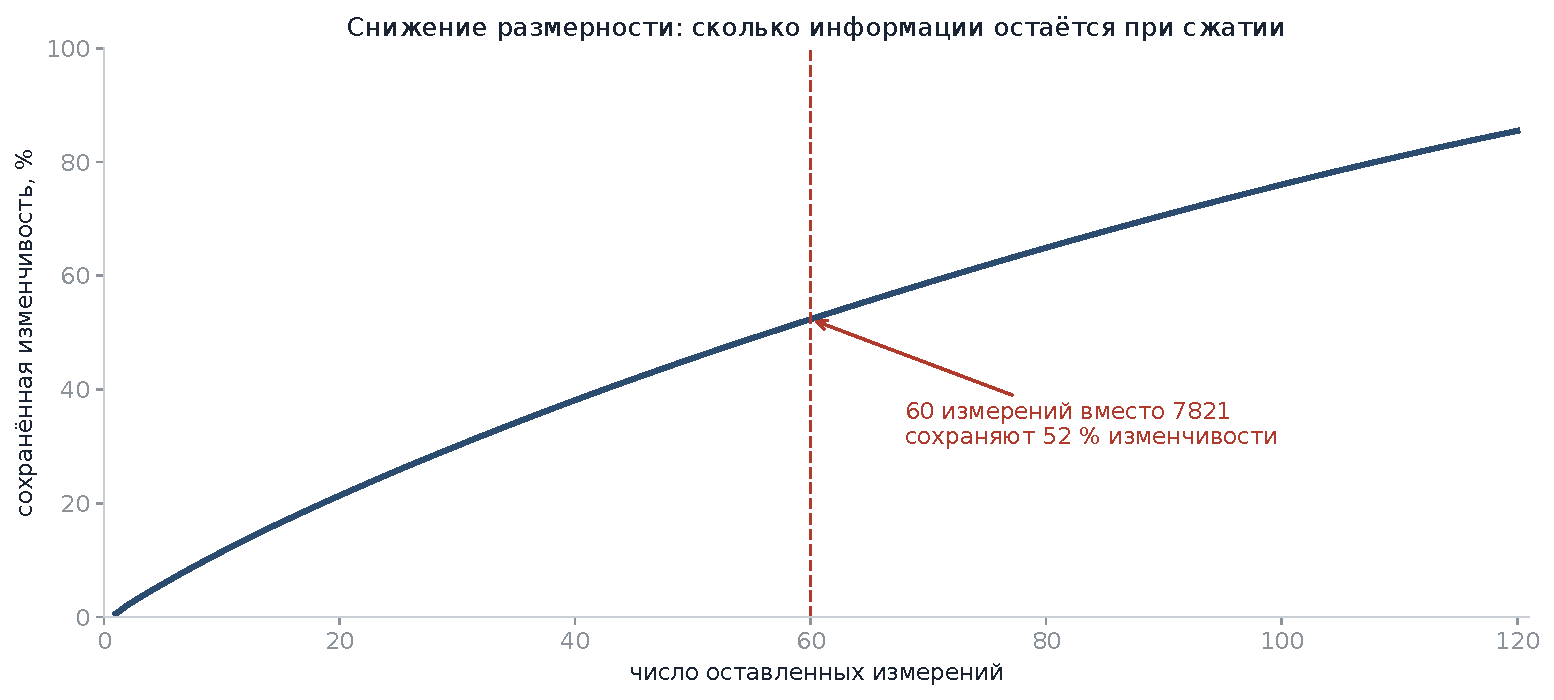
\includegraphics[width=0.62\textwidth]{fig/svd.pdf}
  \end{center}

  \vspace{-0.6em}
  {\small Символьные n-граммы дают \числ{7821} признак — больше, чем
  сегментов в корпусе. SVD оставляет 60 направлений, вдоль которых сегменты
  различаются сильнее всего, и сохраняет \числ{52~\%} изменчивости.}

  \vspace{0.5em}
  \врезка{Сжатие не добавляет знания о языке: оно убирает шум, а вместе с
  ним часть сигнала. LSA не выиграл ни одного запроса у символьных n-грамм,
  из которых он получен.}
\end{frame}

% =====================================================================
\begin{frame}{13 запросов: где меры расходятся}
  Каждый запрос — это эталонный сегмент с одной намеренной правкой.
  Левенштейн и символьные n-граммы дают один и тот же ответ на \числ{9}
  запросах из \числ{13}.

  \vspace{0.9em}
  \begin{columns}[T,onlytextwidth]
    \column{0.47\textwidth}
      {\color{moss}\bfseries Меры согласны — 9 запросов}\\[0.5em]
      {\small добавлено слово\par
      заменён термин\par
      изменено число\par
      заменена концовка\par
      похожего сегмента нет}
    \column{0.47\textwidth}
      {\color{brick}\bfseries Меры расходятся — 4 запроса}\\[0.5em]
      {\small переставлены слова\par
      номинализация\par
      короткий сегмент внутри длинного\par
      синонимия без общих слов}
  \end{columns}

  \vspace{1.0em}
  \врезка{Совпадение на девяти запросах не означает, что мера не важна:
  это означает, что девять правок были простыми. Работа — про четыре
  оставшихся.}
\end{frame}

% =====================================================================
\begin{frame}{Расхождение 1: порядок слов}
  \begin{columns}[T,onlytextwidth]
    \column{0.47\textwidth}
      {\small
      Запрос: {\color{navy}\bfseries «Настройки поиска»}\par
      \vspace{0.8em}
      {\color{brick}Левенштейн} $\rightarrow$ «Начните за три простых
      шага.» \quad \числ{28{,}6~\%}\par
      \vspace{0.6em}
      {\color{moss}n-граммы} $\rightarrow$ «Поиск по настройкам»
      \quad \числ{0{,}696}}
    \column{0.47\textwidth}
      {\color{navy}\bfseries Почему}\\[0.4em]
      {\small Для Левенштейна перестановка слов — это почти полная
      перезапись строки. Он честно находит ближайшее по символам, и это
      случайный сегмент.\par
      \vspace{0.6em}
      Мешок n-грамм порядка не видит вовсе — и именно поэтому выигрывает.}
  \end{columns}

  \vspace{0.7em}
  \врезка{Слепота к порядку слов здесь оказалась достоинством. В другой
  задаче она же будет дефектом — «собака укусила человека» и «человек
  укусил собаку».}
\end{frame}

% =====================================================================
\begin{frame}{Расхождения 2 и 3: оба ответа защитимы}
  \begin{columns}[T,onlytextwidth]
    \column{0.47\textwidth}
      {\small
      {\color{navy}\bfseries Номинализация}\par
      Запрос: «Сохранение изменений»\par
      \vspace{0.5em}
      Левенштейн $\rightarrow$ «Сохранить изменения» \числ{75{,}0~\%}\par
      n-граммы $\rightarrow$ «Изменения сохранены» \числ{0{,}760}\par
      \vspace{0.6em}
      Оба сегмента уместны, различаются грамматикой. Выбирает человек.}
    \column{0.47\textwidth}
      {\small
      {\color{navy}\bfseries Короткий сегмент в длинном запросе}\par
      Запрос: «Пожалуйста, очистите кэш и повторите попытку»\par
      \vspace{0.5em}
      Левенштейн $\rightarrow$ мимо \числ{29{,}5~\%}\par
      n-граммы $\rightarrow$ «Очистить кэш» \числ{0{,}591}\par
      \vspace{0.6em}
      Левенштейн делит на длину — длинный запрос штрафуется сам по себе.}
  \end{columns}

  \vspace{0.7em}
  \врезка{Ни одна из мер не «ошиблась». Они отвечают на разные вопросы, и
  вопрос выбирает тот, кто настраивает инструмент.}
\end{frame}

% =====================================================================
\begin{frame}{Расхождение 4: синонимия}
  \begin{columns}[T,onlytextwidth]
    \column{0.47\textwidth}
      {\small
      Запрос: {\color{navy}\bfseries «По вашему запросу результатов нет»}\par
      Нужный ответ: {\color{moss}\bfseries «Ничего не найдено»}\par
      \vspace{0.8em}
      Общих слов — ноль. Поэтому:\par
      \vspace{0.4em}
      Левенштейн — не находит\par
      n-граммы — не находит\par
      LSA — не находит\par
      \vspace{0.5em}
      {\small Ни один из трёх не ставит нужный сегмент даже в первую тройку.}}
    \column{0.47\textwidth}
      {\color{brick}\bfseries Готовые эмбеддинги}\\[0.4em]
      {\small Находят — на \числ{2-м} месте. Первым идёт другой сегмент.\par
      \vspace{0.7em}
      Это честный результат работы: средство, которое должно было решить
      проблему, решает её \emph{не до конца}.\par
      \vspace{0.7em}
      В CAT-инструменте это значит, что подсказка будет — но переводчику
      придётся её заметить среди других.}
  \end{columns}

  \playground{https://konkin-nikita.ru/gd_learn/tm/}{память переводов}%
  {этот запрос можно прогнать всеми четырьмя мерами сразу.}
\end{frame}

% =====================================================================
\begin{frame}{Порог 75~\% — это решение, а не настройка}
  \begin{columns}[T,onlytextwidth]
    \column{0.46\textwidth}
      {\small
      \begin{tabular}{@{}rrr@{}}
        \toprule
        порог & подсказок & верных \\
        \midrule
        60~\% & 10 & 9 \\
        70~\% & 9 & 8 \\
        \textbf{75~\%} & \числ{7} & 6 \\
        80~\% & 5 & 5 \\
        90~\% & 2 & 2 \\
        \bottomrule
      \end{tabular}\par
      \vspace{0.5em}
      Из 13 запросов.}
    \column{0.48\textwidth}
      {\small
      Отраслевой порог в 75~\% на этих запросах прячет почти половину
      памяти: подсказка есть, но переводчик её не увидит.\par
      \vspace{0.7em}
      Поднять порог до 90~\% — остаётся \числ{2} подсказки из 13, зато обе
      верные.\par
      \vspace{0.7em}
      {\color{brick}\bfseries Это компромисс, а не оптимум.} Что дороже —
      пропущенная подсказка или подсказка, которую придётся править, —
      знает менеджер проекта, а не алгоритм.}
  \end{columns}
\end{frame}

% =====================================================================
\begin{frame}{Второй отрицательный результат: кластеризация}
  Если сегменты хорошо представлены числами, похожие должны собираться
  вместе сами — без разметки. Совпадут ли кластеры с типами контента?

  \vspace{0.5em}
  {\small
  \begin{tabular}{@{}l@{\hspace{2em}}r@{\hspace{2em}}l@{}}
    \toprule
    представление & ARI & разброс по восьми запускам \\
    \midrule
    символьные n-граммы & 0,079 & 0,015 -- 0,079 \\
    LSA                 & 0,043 & 0,017 -- 0,122 \\
    готовые эмбеддинги  & 0,172 & 0,143 -- 0,234 \\
    \bottomrule
  \end{tabular}}

  \vspace{0.6em}
  {\small ARI = 1 — кластеры совпали с разметкой, ARI = 0 — совпали
  случайно. {\color{brick}\bfseries Все три числа близки к нулю:}
  кластеризация находит длину, наличие цифр и формат, а не тип контента.}

  \vspace{0.6em}
  \врезка{\textbf{Это правильный результат, а не поломка.} Тип контента
  придуман людьми для бизнес-процесса — данные не обязаны о нём знать.}
\end{frame}

% =====================================================================
\begin{frame}{Как это выглядит}
  \begin{center}
    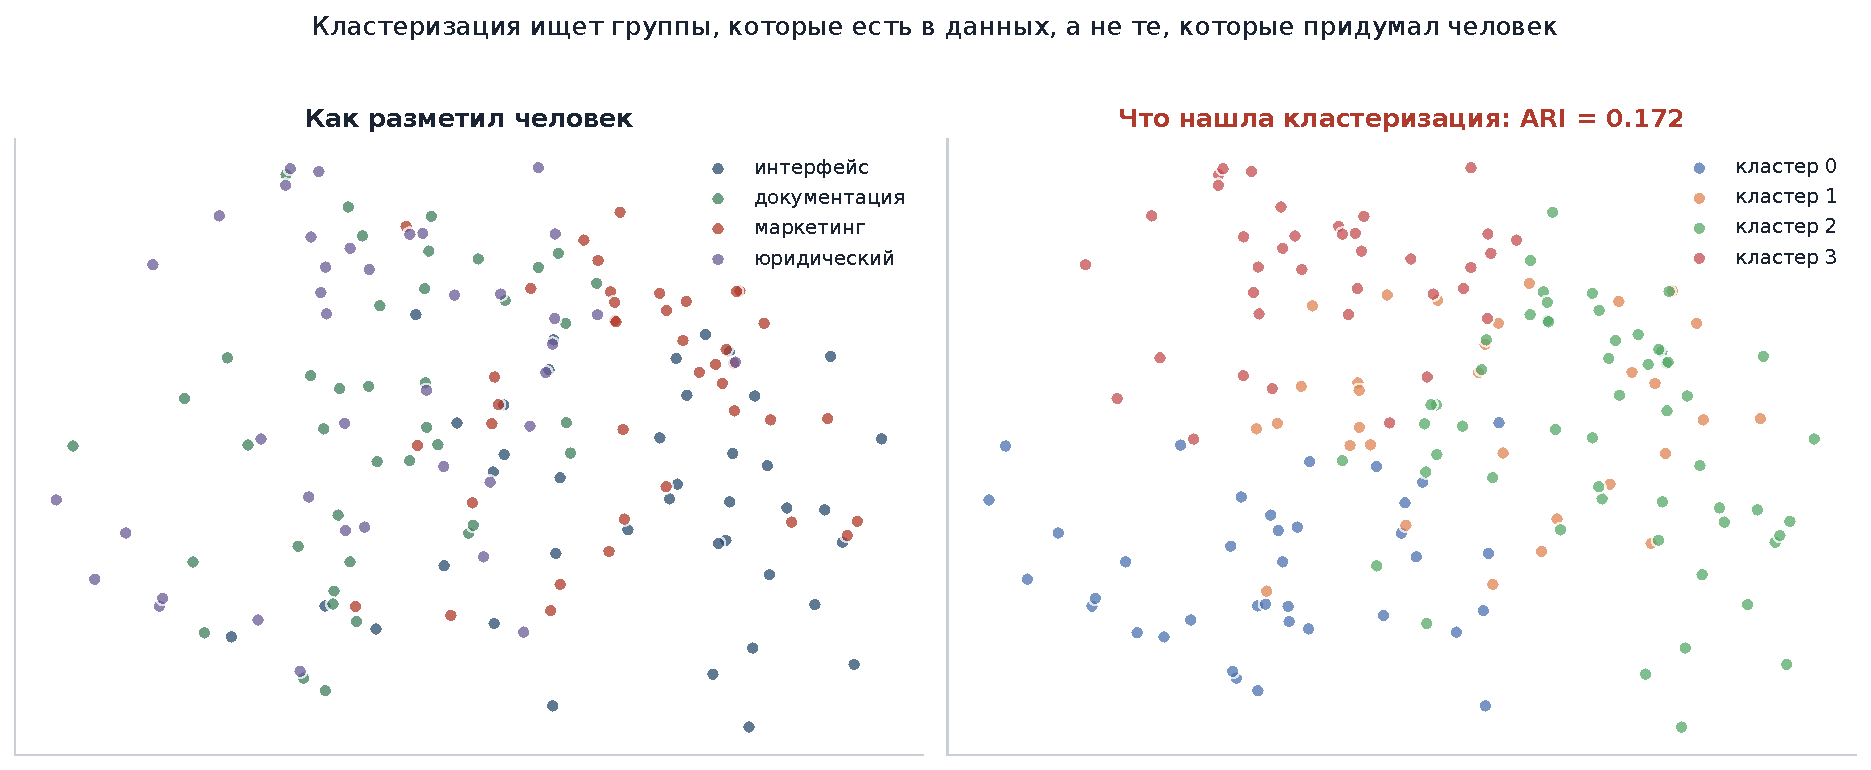
\includegraphics[width=0.93\textwidth]{fig/clusters.pdf}
  \end{center}

  \vspace{-0.3em}
  {\small Слева — разметка по типам контента, справа — что нашла
  кластеризация на готовых эмбеддингах, лучшем из трёх представлений.
  Границы не совпадают нигде: {\color{brick}\bfseries кластеры реальны, но
  это не типы контента.}}
\end{frame}

% =====================================================================
\begin{frame}{Почему ARI нельзя приводить с тремя знаками}
  \begin{columns}[T,onlytextwidth]
    \column{0.47\textwidth}
      {\small
      Разброс по восьми запускам у символьных n-грамм: от \числ{0{,}015}
      до \числ{0{,}079}.\par
      \vspace{0.7em}
      Это \emph{шире}, чем разница между символьными n-граммами и LSA.\par
      \vspace{0.7em}
      Кроме того, k-means на разреженной матрице приходит к разному
      локальному минимуму в зависимости от библиотеки линейной алгебры:
      на одной машине 0,079, на другой 0,023.}
    \column{0.47\textwidth}
      {\color{brick}\bfseries Что из этого следует}\\[0.4em]
      {\small Число в три знака здесь описывает не корпус, а версию
      библиотеки и номер запуска.\par
      \vspace{0.7em}
      В отчёте про кластеризацию корректно писать: «ARI около нуля при
      любом из представлений; разброс между запусками шире разницы между
      ними».\par
      \vspace{0.7em}
      Так сформулированное утверждение воспроизводится где угодно.}
  \end{columns}

  \playground{https://konkin-nikita.ru/gd_learn/tm/}{память переводов}%
  {вкладка «Кластеризация» показывает ARI вместе с разбросом по запускам.}
\end{frame}

% =====================================================================
\begin{frame}{Что должно быть в отчёте}
  \begin{columns}[T,onlytextwidth]
    \column{0.47\textwidth}
      {\color{moss}\bfseries Обязательно}\\[0.5em]
      {\small
      1. Разбор всех четырёх расхождений: какая мера что нашла и почему.\par
      \vspace{0.4em}
      2. Вывод про порог: что он прячет и чем за это платят.\par
      \vspace{0.4em}
      3. Оба отрицательных результата — синонимия и кластеризация — с
      объяснением, почему они закономерны.}
    \column{0.47\textwidth}
      {\color{brick}\bfseries Типичная ошибка}\\[0.5em]
      {\small Объявить меру-победителя. Её нет.\par
      \vspace{0.7em}
      Символьные n-граммы выигрывают три расхождения из четырёх — и
      проигрывают там, где порядок слов важен. Эмбеддинги решают
      синонимию — и требуют чужой предобученной модели, которая ничего не
      знает о терминологии вашего проекта.}
  \end{columns}
\end{frame}

% =====================================================================
\begin{frame}{Что унести из работы № 2}
  \begin{columns}[T,onlytextwidth]
    \column{0.47\textwidth}
      {\color{navy}\bfseries Про представления}\\[0.5em]
      {\small «Похоже» — не свойство пары текстов, а свойство выбранной
      меры. Смена представления меняет ответ, а не уточняет его.\par
      \vspace{0.6em}
      Отрицательный результат — тоже результат, если объяснено, почему он
      закономерен.}
    \column{0.47\textwidth}
      {\color{brick}\bfseries Про профессию}\\[0.5em]
      {\small Процент совпадения в вашем CAT-инструменте — это чьё-то
      решение о мере и о пороге. Теперь вы знаете, какое именно, и можете
      спорить о нём по существу.}
  \end{columns}

  \vspace{1.2em}
  \playground{https://konkin-nikita.ru/gd_learn/tm/}{память переводов}%
  {все 13 запросов, четыре меры, порог и кластеризация — в браузере.}
\end{frame}

\end{document}
